\documentclass[fleqn, 10pt]{wlscirep}
\usepackage[utf8]{inputenc}
\usepackage[T1]{fontenc}
\usepackage{textcomp}
\usepackage{gensymb}
\usepackage{textgreek}
\usepackage{authblk}
\usepackage{amsmath}
\setcounter{figure}{0}
\makeatletter 
\renewcommand{\thefigure}{S\@arabic\c@figure}
\makeatother
\title{Dynamics of a neuronal pacemaker in the weakly electric fish \emph{Apteronotus}}

\author[1,2,3*]{Aaron R. Shifman}
\author[1,2,3]{Yiren Sun}
\author[1,2,3]{Chloé M. Benoit}
\author[1,2,3]{John E. Lewis}
\affil[1]{Department of Biology, University of Ottawa, Ottawa, Ontario, Canada K1N 6N5}
\affil[2]{Center for Neural Dynamics, University of Ottawa, Ottawa, Ontario, Canada K1N 6N5}
\affil[3]{uOttawa Brain and Mind Research Institute, Ottawa, Ontario, Canada K1H 8M5}
\affil[*]{ashifman@uottawa.ca}

\renewcommand\Affilfont{\itshape\small}
\begin{document}
	\maketitle
	\begin{figure}[!ht]
	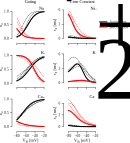
\includegraphics[scale=1]{../figures/fs1}
	\caption{Voltage-dependence functions for each model current across all model fits. Thick lines represent canonical model in figure 1C(i) and dashed lines represent models in figure 1C(ii-iv). Gating functions (left) and time constant functions (right) with rows representing functions for sodium, potassium, and calcium descending.}
	\end{figure}
\end{document}   
